\subsection{Memoria Principal y Memoria Caché}

	En la primera parte de ésta serie de papers, logramos ver que 
las operaciones aritméticas más comunes, toman entre 1 a 10 ciclos de 
CPU. Sin embargo, para poder realizar estas operaciones, es necesario
 contar con el medio de almacenamiento necesario para los datos utilizados
 en cada operación, por lo que se hace primordial, tener en consideración 
el acceso a este medio. El acceso a la memoria principal puede tomar
 aproximadamente unos 300 ciclos de CPU, por lo que si se desarrollan 
algoritmos optimizados, todo el esfuerzo es en vano si el acceso a la 
memoria principal produce grandes latencias.\\\\
	Para suerte de nosotros, los diseñadores de hardware han desarrollado
 estrategias para cubrir este gran problema, para ello decidieron colocar una
 pequeña memoria en una posición muy cercana al CPU, a la cual denominan memoria
 caché, las cuales poseen una característica importante, ser extremadamente 
rápida. Con esta disposición, los datos son accesados mucho mas rápida que si
 fueran leídos desde la memoria principal. Los procesadores más modernos poseen 
dos o más niveles de caché, denominados L1,L2 y así sucesivamente, los que dan 
a tranzar entre tamaño y velocidad. Leer desde la memoria cache L1 es muy rápido
 comparado con la memoria principal, pero a su vez tiene mucha menos capacidad 
de almacenamiento.\\\\
	La principal tarea de los programadores, es entonces, lograr un 
entendimiento sólido en este aspecto, para de esta forma llegar a comprender
 en que condiciones los datos son almacenados en la memoria caché y así lograr
 asegurar que los datos que necesitemos, se encuentren en ella.

\subsection{Localidad}

Primero que todo debemos comprender que el cache funciona \emph{reteniendo los datos utilizados recientemente},
para poder obtenerlos mas rápido en una próxima situación.
Obviamente no es posible retener los datos por un tiempo indefinido,
por lo cual son retenidos el máximo tiempo posible y van a salir de la memoria cache,
solo cuando otros datos necesiten ser retenidos.

Por lo tanto el paper analizado nos plantea que una forma de reducir la frecuencia de tener que ir a la memoria principal en variadas ocasiones,
es reutilizar los datos todas las veces que sea posible posible dentro de un periodo de tiempo corto,
porque los datos seguirán estando en el cache y no tendremos que hacer todo el procedimiento de nuevo

El concepto anteriormente señalado es conocido como \emph{localidad temporal}

Como hablamos de \emph{localidad temporal},
también es necesario tocar el tema de la \emph{localidad espacial},
la cual corresponde a cuando un programa usa múltiples partes de datos que han sido guardados contiguos en un periodo corto de tiempo.
El ejemplo que el paper ilustra de localidad espacial,
facilita la comprensión, éste nos señala una simple situación de recorrer un arreglo secuencialmente.

Por otro lado el cache aprovecha la \emph{localidad espacial} recuperando y almacenando toda la secuencia de bytes contiguos,
es decir, no sólo los bytes específicos de los datos solicitados por el procesador.
\emph{¿Cuál es la idea de recuperar y almacenar toda la secuencia de bytes?}
Claramente es poder satisfacer futuras solicitudes de direcciones de memoria cercana.

Hay otra forma en la cual una \emph{localidad espacial} de programas puede mejorar el desempeño del cache,
esta se basa en aspecto del funcionamiento del cache.
Si todo fuera perfecto cualquier linea de datos podría estar en una linea de cache,
pero para poder limitar el numero de lineas que deben ser buscadas y poder conservar los tiempos de acceso al cache cortos,
el mismo cache se preocupa de limitar las lineas de cache donde pueden estar las lineas de datos.

\begin{center}
	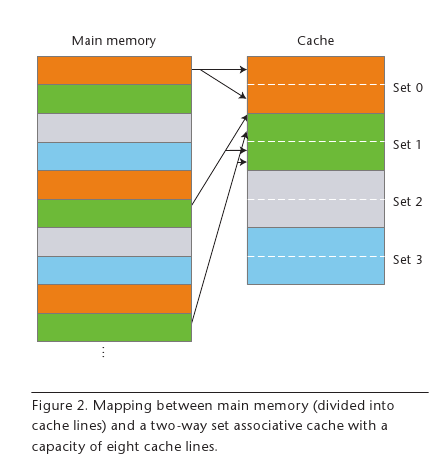
\includegraphics[scale=0.7]{images/figura2}
\end{center}

Las áreas verdes en la memoria principal pueden mapear solo una de dos lineas de cache verdes en el cache.
Si mas de dos áreas mapean el mismo conjunto,
resulta un conflicto, causando que algunos datos sean desalojados.

El conflicto de que dos áreas mapeen el mismo conjunto puede ser evitado con ayuda de la \emph{localidad espacial},
porque áreas contiguas en la memoria principal garantizan un mapeo a diferentes conjuntos en el cache.

\subsection{Mejorando la localidad espacial: \emph{Array-Merging}}
Esta Técnica, \emph{Array-Merging}, se utiliza para mejorar el tiempo de acceso a los datos en la \emph{memoria principal}.
En el ejemplo, se declaran los siguientes arreglos:
\begin{lstlisting}[language=C]
 int x[N], y[N];
 float sin6[N], cos6[N];
 int count[MAX_R];
 float g[MAX_R];
\end{lstlisting}

\begin{center}
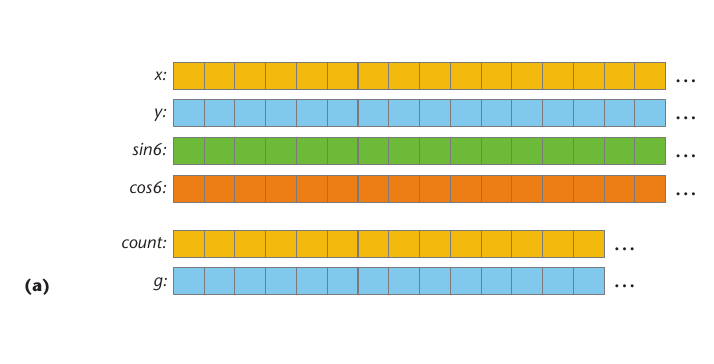
\includegraphics[scale=0.6]{images/array-1.png}
\end{center}

Si bien esto mejora el tiempo de acceso a los datos, solo sirve para requerimientos de los arreglos, ya sea $x[N]$ o $y[N]$, pero en el programa necesitamos acceso a el elemento \emph{n-esimo} de los 4 arreglos de input y el elemento \emph{r-esimo} de los 2 arreglos de output al mismo tiempo. Para mejorar la localidad espacial usamos el método del que hablamos, \emph{Array-Merging}, que guarda los valores, asociado a cada \emph{n-esimo} elemento, de forma contigua. 
Para poder llevar a cabo esta técnica podemos utilizar C, donde debemos definir estructuras donde poner cada uno de nuestros arreglos. Con esto cada vez que la memoria Cache necesite los valores, de manera anexa, también guardara los demás valores que serán necesarios. Esto lo podemos ver en el siguiente código.

\begin{lstlisting}[language=C]
struct DataStruct {
 int x, y;
 float cos6, sin6; };
DataStruct data[N];
struct AccumulationStruct {
 int count;
 float g; };
AccumulationStruct accum[Max_R];

//Now, accumulate data for all pairs of
//points (i,j).
for(i=0; i<N; ++i) //for each i < N
 for(j=i+1; j<N; ++j) { //for each j < N
  Dx = data[i].x - data[j].x;
  Dy = data[i].y - data[j].y;
  r = sqrt(Dx*Dx + Dy*Dy);
  accum[r].g += data[i].cos6 * data[j].cos6 +
   data[i].sin6 * data[j].sin6;
  ++accum[r].count;
}
\end{lstlisting}


\begin{center}
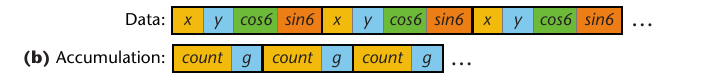
\includegraphics[scale=0.6]{images/array-2.png}
\end{center}

\subsection{Mejorando la localidad temporal: \emph{Blocking}}

La idea de mejorar la localidad temporal, es la de mantener los datos más recientemente accedidos
``cercanos'' al procesador.

El método consiste en agrupar las variables de entrada en pequeños bloques (del tamaño
\emph{blocksize}) que quepa fácilmente en el cache de menor nivel. Entonces, podemos procesar cada
par posible de puntos de esos dos bloques antes de pasar a procesar el siguiente par de bloques.
% como muestra la figura 4(...).
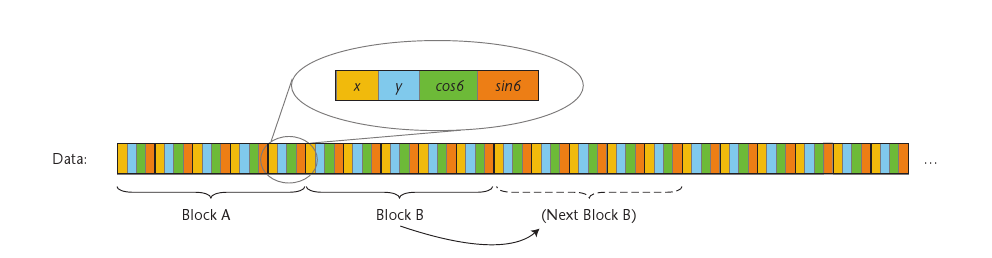
\includegraphics[scale=0.7]{images/figure4}

De esta forma, se logran realizar más computaciones por cada nuevo punto de información leído de la
memoria principal. Por ejemplo, si guardamos en el caché dos bloques de información, cada uno con un
tamaño de 100 puntos, podríamos procesar todos los 10.000 pares de puntos posibles antes de tener que
acceder al siguiente bloque de 100 puntos, lo cual es una gran mejora comparada con procesar un solo par
de puntos por cada punto leído.

La porción de código modificado queda como sigue:\\
\scriptsize
\begin{lstlisting}[language=C]
for(A = 0; A+2*blocksize < N; A+= blocksize)
	for(B=A+blocksize; B+blocksize<N; B+=blocksize)
		for(i=A; i<A+blocksize; ++i)
			for(j=B; j<B+blocksize; ++j)
			{
				(...)
			}
(...)
\end{lstlisting}
\normalsize
La desventaja de esta técnica consiste en que el código se vuelve más complejo y necesita la
implementación de más código para le manejo de nuevos casos especiales (rangos fuera de índices y evitar
que falten o se repitan operaciones).\\
 Si vemos el código, nos damos cuenta que aumentamos el número de iteraciones anidadas de 2 a 4.
Además, este no incluye los casos especiales para que funcione.\\

Por ello, nos vimos obligados a implementar nuestro própio código para probar el método de ``blocking''
en el algoritmo:
\scriptsize
\begin{lstlisting}[language=C]
	for(A=0; A<N; A+=blocksize)
	{
		C=A;
		for(B=A,flag=1; B<N; B+=blocksize,flag=0)
		{
			for(i=A; i<A+blocksize; ++i)
			{	
				if(flag)
				{
					C++;
					for(j=C; j<B+blocksize; ++j)
					{
						(...)
					}
				}
				else
					for(j=B; j<B+blocksize; ++j)
					{
						(...)
					}
			}
			C=B;
		}
	}
(...)
\end{lstlisting}
\normalsize


\textbf{Resultados}\\
En los casos de prueba  aumentó el tiempo de procesamiento en comparación con el código original.\\
Posibles causas de este resultado:
\begin{itemize}
        \item Nuestro hardware ya estaba haciendo un excelente trabajo.
        \item El aumento de operaciones por cada ciclo no se compensaba
\end{itemize}

Para más información del código utilizado, ver los anexos.

\subsection{Mejoras propuestas en nuestra investigación}
\subsubsection{Aproximación de raíces}

Utilizaremos una \emph{lookup table}, la cual es una estructura de datos, usualmente un arreglo o un arreglo asociativo.
Esta tabla es usada para reemplazar un cálculo en tiempo de ejecución,
con una simple operación de indexación de un arreglo.

Por lo tanto nos remontamos al siguiente \emph{código}:

\textbf{Original}
\begin{center}
\begin{lstlisting}[language=C]
...
for(j=i+1;j<N;++j)
{
	Dx = data[i].x - data[j].x;
	Dy = data[i].y - data[j].y;
	r = sqrt(Dx*Dx + Dy*Dy);
	accum[r].g+=data[i].cos6 + data[j].cos6 +data[i].sin6 + data[j].sin6;
	++accum[r].count;
}
...
\end{lstlisting}
\end{center}
\textbf{Modificado}
\begin{center}
\begin{lstlisting}[language=C]
...
for(j=i+1;j<N;++j)
{
	Dx = data[i].x - data[j].x;
	Dy = data[i].y - data[j].y;
	root(Dx*Dx + Dy*Dy, r)
	accum[r].g+=data[i].cos6 + data[j].cos6 +data[i].sin6 + data[j].sin6;
	++accum[r].count;
}
...
\end{lstlisting}
\end{center}

Nuestra función \emph{root()} la hemos implementado aparte en un archivo \emph{.h};
el cual no es nada más que un \emph{switch} con muchos \emph{case}.

\begin{center}
\begin{lstlisting}[language=C]
#define root(x,y)
	switch(x){
	case 0: y = 0; break;
	case 1: y = 1; break;
	case 2: y = 1; break;
	case 3: y = 1; break;
	...
	case 997: y = 31; break;
	case 998: y = 31; break;
	case 999: y = 31; break;
	}
\end{lstlisting}
\end{center}

Lo cual nos sirve para poder acceder a \emph{aproximaciones} de valores,
en vez de tener que calcular la raíz de un determinado numero.

Obviamente en la vida real,
se utilizan tablas mucho mas grandes.


\subsubsection{Aproximación de funciones trigonométricas}
Como en nuestro código realizamos muchos cálculos de \emph{funciones trigonométricas},
tenemos como motivación poder optimizar el tiempo y cálculo de éstas.

Podemos recordar las \emph{Series de Taylor}, para realizar una suerte de aproximación.

$$\sin{x} = \sum^{\infty}_{n=0} \frac{(-1)^n}{(2n+1)!} x^{2n+1} = x - \frac{x^3}{3!} + \frac{x^5}{5!} - \ldots \forall x$$

El problema radica en que algunos computadores, no pueden calcular el \emph{seno} de un valor dado,
pues están limitados a realizar operaciones básicas.

Las series de Taylor nos brindan una herramienta para poder calcular ciertas funciones trigonométricas,
con una gran presición.

Ocuparemos entonces una aproximación para calcular el \emph{seno}:

$$\sin{x} \approx x - \frac{x^3}{6} + \frac{x^5}{120} - \frac{x^7}{5040}$$

Pero, ocupamos muchas multiplicaciones para calcular los $x^k$,
por lo cual utilizaremos el \emph{Algoritmo de Horner}.

Éste algoritmo plantea una forma de calcular eficientemente polinomios de una forma monomial,
es decir,
$$ p(x) = a_0 + a_1 x + a_2 x^2 + a_3 x^3 + \cdots + a_n x^n $$

Por lo tanto podremos reducir nuestro polinomio:
$$\operatorname{sin}(x) \approx x - \frac{x^3}{6} + \frac{x^5}{120} - \frac{x^7}{5040}$$
		a,
$$\operatorname{sin}(x) \approx x \left( 1 - x^{2}\left(\frac{1}{6} + x^{2}\left(\frac{1}{120} - \frac{x^2}{5040}\right)\right)\right)$$

Si nos damos cuenta estamos reduciendo el número de multiplicaciones de 12 a 3

Luego de varias pruebas en el cálculo de efectuar ésta operación,
nos dimos cuenta que se transforma en un cálculo muy caro,
especialmente para procesadores lentos.

\subsection{Pruebas}
\subsubsection{Justificación}

Actualmente casi todos contamos con computadores con una capacidad respetable en comparación a las últimas tecnologías existentes,
pero estamos descuidando un área muy popular, los cuales son los sistemas embebidos.

Es por eso que en nuestro trabajo hemos optado por trabajar con un equipo con arquitectura ARM\footnote{http://es.wikipedia.org/wiki/ARM},
pues su capacidad de procesamiento es mucho menor, pero aspira alcanzar procesamientos al mismo nivel que un computador normal.
Si nos damos cuenta, la mayoría de los dispositivos como celulares, pocketpc, netbooks, etc, poseen poca memoria y necesitan que cada operación que se realice
sobre ella sea lo más óptima posible.

Finalmente,
una mejora en un algoritmo en un computador de escritorio o notebook actual, quizás no podremos notar la diferencia,
pero en sistemas embebidos pueden significar un gran ahorro de tiempo y provocar un mayor desempeño.

\subsubsection{Hardware}

	El kit de desarrollo Intrinsyc's Cerf$^{TM}$Board 250 provee una plataforma 
flexible, con hardware y software de alto desempe\~no para desarrollar aplicaciones 
embebidas en forma r\'apida. El kit incluye:

\begin{itemize}
	\item Intel PXA250 (XScale)
	\item Tarjeta de expansi\'on Cerf IO 250
	\item Tarjeta de expansi\'on CerfComm 250
	\item Intrinsyc's I-Linux con kernel 2.4
\end{itemize}

\begin{center}
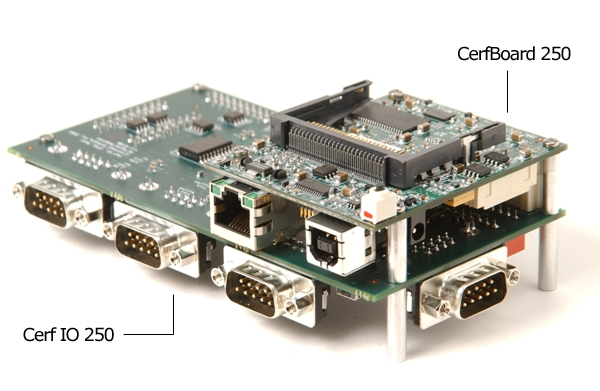
\includegraphics[scale=0.3]{images/board}
\end{center}

\subsubsection{Intel PXA250 (XScale)}

	El Intel PXA250 es un microprocesador basado en un n\'ucleo Intel XScale.
Intel XScale es una micro arquitectura RISC de 32-bit basado en una arquitectura ARM. Dise\~nado para un alto desempe\~no a costa de usar poca energ\'ia. Incorpora un conjunto completo de sistemas y perif\'ericos, funciones que le permite ser utilizado en una variedad de port\'atiles de mano.

	Posee las siguientes caracter\'isticas t\'ecnicas:

\begin{itemize}
	\item Frecuencia de 400MHz
	\item Memoria Principal de 64MB
	\item Cach\'e de instrucciones de 32KB
	\item Cach\'e de datos de 32KB
	\item B\'ufer de 256 bit
	\item Controlador de memoria basado en una arquitectura de memoria unificada, donde todos los dispositivos de memoria externos comparten un bus de direcci\'on y datos en com\'un.
	\item El controlador de memoria consiste en cuatro unidades de control principal para dar interfaz a memorias din\'amicas (SDRAM), memorias est\'aticas (ROM, SRAM, Flash), PCMCIA y chips similares.
	\item La memoria externa es vista como una colecci\'on lineal de bytes numerados desde 0 hacia adelante.
\end{itemize}

\begin{center}

\includegraphics[scale=0.5]{images/pxa250}
\end{center}

\subsubsection{Tarjeta de expansi\'on Cerf IO 250}

	La tarjeta de expansi\'on Cerf IO 250 es una placa con entrada y salida
de propósito general. Viene equipada con un puerto serial de depuraci\'on RS232,
dos puertos seriales RS232, un puerto serial RS422/485, entre otros.

\subsubsection{Tarjeta de expansi\'on CerfComm 250}

	La tarjeta de expansi\'on CerfComm 250 est\'a equipada con caracter\'isticas
en la comunicaci\'on, viene con un controlador USB Host, un puerto Ethernet  10/100
 y tres puertos seriales de depuraci\'on RS232.

\subsubsection{Resultados}

	Para la realización de las pruebas consideramos una cantidad de datos 
igual a 50000, por otro lado programamos dos ejemplos, el primero de ellos consiste 
en la implementación mas rápida de codificar, sugerida por los papers, mientras 
que el segundo ejemplo incluye las optimizaciones sugeridas,
a continuación los resultados:\\

\begin{tabular}{|l|l|l|l|l|}
\hline
& Normal & Optimización 1 & Optimización 2 & Optimización 3 \\
\hline
Tiempo ejecución [s] & 143 & 55 & 54 & 54\\
\hline
\end{tabular}

\begin{itemize}
	\item Optimización 1: Calculo previo de funciones trigonométricas
	\item Optimización 2: Array merging
	\item Optimización 3: Blocking
\end{itemize}


